\documentclass[14pt,a4paper,oneside]{article}

\usepackage[utf8x]{inputenc}
\usepackage[warn]{mathtext}
\usepackage{amsmath}
\usepackage[russian]{babel}
\usepackage{fontspec} 
\setmainfont{Times New Roman}
\usepackage[14pt]{extsizes}
\usepackage{tabularx}
\usepackage{microtype}
\usepackage{verbatim}
\usepackage{longtable}
\usepackage{ccaption}
\usepackage{multirow}
\usepackage{url}
\usepackage{array}
\usepackage{longtable}

\usepackage{graphicx}
\DeclareGraphicsExtensions{.pdf,.png,.jpg}

\usepackage[top=2cm,bottom=2cm,left=3cm,right=1cm]{geometry}
\newcolumntype{C}[1]{>{\hsize=#1\hsize\centering\arraybackslash}X}%
\newcolumntype{P}[1]{>{\centering\arraybackslash}p{#1}}

\usepackage{ragged2e}
\justifying
\sloppy
\tolerance=500
\hyphenpenalty=10000
\emergencystretch=3em

\newlength{\fivecharsapprox}
\setlength{\fivecharsapprox}{1.5cm}

\usepackage{indentfirst}
\setlength{\parindent}{1.5cm} % для шрифта 14pt

%\renewcommand{\rmdefault}{ftm}

\usepackage{fancyhdr} % пакет для установки колонтитулов
\pagestyle{fancy} % смена стиля оформления страниц
\fancyhf{} % очистка текущих значений
%\rfoot{\normalsize \thepage} % установка верхнего колонтитула
\fancyfoot[R]{\normalsize \thepage}
\renewcommand{\footrulewidth}{0pt} % убрать разделительную линию внизу страницы
\renewcommand{\headrulewidth}{0pt} % убрать разделительную линию вверху страницы

% SECTION
\makeatletter
\renewcommand\section{%
  \@startsection {section}{1}%
    {\fivecharsapprox}%
    {-1em \@plus -1ex \@minus -.2ex}%
    {1em \@plus .2ex}%
    {\raggedright\centering\hyphenpenalty=10000\normalfont\normalsize\bfseries\MakeUppercase}}
\makeatother

% SUBSECTION
\makeatletter
\renewcommand\subsection{%
  \@startsection{subsection}{2}%
    {\fivecharsapprox}%
    {-1em \@plus -1ex \@minus -.2ex}%
    {1em \@plus .2ex}%
    {\raggedright\hyphenpenalty=10000\normalfont\normalsize\bfseries}}
\makeatother

% REFERENCES
\makeatletter
\renewcommand\@biblabel[1]{#1.}
\makeatother

% FIGURES AND TABLES
\usepackage[tableposition=top]{caption}
\usepackage{subcaption}
\DeclareCaptionLabelFormat{gostfigure}{Рисунок #2}
\DeclareCaptionLabelFormat{gosttable}{Таблица #2}
\DeclareCaptionLabelSeparator{gost}{~---~}
\captionsetup{labelsep=gost}
\captionsetup[figure]{labelformat=gostfigure}
\captionsetup[table]{justification=justified, labelformat=gosttable}
\renewcommand{\thesubfigure}{\asbuk{subfigure}}

%\DeclareCaptionLabelSeparator{fill}{\hfill}
%\DeclareCaptionLabelFormat{fullparents}{\bothIfFirst{#1}{~}#2}
%\DeclareCaptionLabelFormat{fullparents}{Таблица #2}
%\captionsetup[table]{
%     labelformat=gosttable,
%     labelsep = gost,
%     labelsep=fill,
%     labelfont=it,
%     textfont=bf,
%     singlelinecheck=false
%     }
     
\usepackage{setspace} 
\setstretch{1.3}
\onehalfspacing

\renewcommand{\thesection}{\arabic{section}.}
\renewcommand{\thesubsection}{\arabic{section}.\arabic{subsection}.}
\renewcommand{\thesubsubsection}{\arabic{section}.\arabic{subsection}.\arabic{subsubsection}.}
\renewcommand{\theequation}{\arabic{equation}}

\setcounter{totalnumber}{10}
\setcounter{topnumber}{10}
\renewcommand{\topfraction}{1}
\renewcommand{\textfraction}{0}

\usepackage{color} %% это для отображения цвета в коде
\usepackage{listings} %% собственно, это и есть пакет listings

\lstset{language=C++,
				frame=tlrb,xleftmargin=\fboxsep,xrightmargin=-\fboxsep, % Рамка, подогнанная к заголовку
				rulecolor=\color{black},
				breaklines=true,
                basicstyle=\ttfamily\footnotesize,,
                keywordstyle=\color{blue}\ttfamily,
                stringstyle=\color{red}\ttfamily,
                commentstyle=\color{green}\ttfamily,
                morecomment=[l][\color{magenta}]{\#}
}

\usepackage{datatool, filecontents}

\DTLsetseparator{;}

\DTLloaddb{variables}{variables.csv}

\newcommand{\var}[1]{% 
     \DTLgetvalueforkey{\getvalue}{value}{variables}{avar}{#1}
     \getvalue
}%


\begin{document}

\thispagestyle{empty}
\begin{center}
\textbf{Министерство науки и высшего образования Российской Федерации}

федеральное государственное автономное образовательное учреждение высшего образования

\textbf{«НАЦИОНАЛЬНЫЙ ИССЛЕДОВАТЕЛЬСКИЙ ТОМСКИЙ ПОЛИТЕХНИЧЕСКИЙ УНИВЕРСИТЕТ»}
\noindent\rule{\textwidth}{1pt}
\end{center}

\noindent Инженерная школа ядерных технологий

\noindent Направление -- Ядерные физика и технологии

\noindent Отделение ядерно-топливного цикла

\vspace{5em}
\begin{center}
\textbf{КУРСОВОЙ ПРОЕКТ}

по дисциплине <<Междисциплинарный проект>>

на тему <<Расчет основных параметров изотопного обмена в разделительном
каскаде при стационарном режиме его работы>>

Вариант 6
\end{center}
\vspace{7em}
\noindent Исполнитель:

\vspace{2em}
\noindent Проверил:

\vspace{10em}
\centering Томск -- 2021
\newpage

\tableofcontents
\newpage

\noindent\textbf{ЦЕЛЬ РАБОТЫ:} провести расчет изменения концентрации $^{7}$Li по колоннам каскада в 
режимах без отбора и с отбором при заданных параметрах его работы.

\section{Теоретическая часть}
\subsection{Основные определения и соотношения}
Одним из наиболее эффективных промышленных методов разделения изотопов 
лёгких элементов (водорода, лития, бора, углерода и др.) является 
физико-химический метод изотопного обмена. Важной особенностью 
физико-химических методов является обратимость элементарного акта разделения 
и двухфазность рабочей системы.

Наиболее удобной рабочей двухфазной системой считается система 
жидкость – газ. Процесс разделения изотопов при этом проводят в 
разделительных колоннах, при непрерывном противоточном движении потоков 
жидкой ($L$) и газовой ($G$) фаз. Поскольку значения констант равновесия, 
летучестей и т. д. для различных изотопнозамещенных форм различно, 
то возникает изотопный эффект, приводящий к изменению содержания данного 
изотопа в разных фазах. Вследствие этого эффекта, характеризуемого величиной 
коэффициента разделения $\alpha$, содержание изотопа в фазе $L$, покидающей 
некоторое сечение колонны II будет отличаться от содержания этого же изотопа 
в фазе $G$, покидающей сечение I:
\begin{equation}
\alpha = \dfrac{c_{2}(1-c_{1})}{c_{1}(1-c_{2})}
\end{equation}
\noindent где $c_{1}, c_{2}$ – мольные доли целевого изотопа в равновесных фазах.

Уравнение, описывающее обогащение в каскаде из элементов второго рода, 
при условии, что $\alpha$ для всех элементов одинаково, а коэффициент 
обогащения $\varepsilon = (\alpha – 1) << 1$ и поток отбора $P << L$ 
имеет вид:
\begin{equation}
\dfrac{dc}{dn} = \varepsilon c(1-c) - \dfrac{P}{L}(c_{P}-c)
\end{equation}
\noindent где $c_{P}$ – концентрация отбора.

\subsection{Принципиальная схема работы колонны или каскада колонн}
Разделительные колонны различаются по виду, особенностям строения и работы. 
На рисунке ~\ref{fig:cascade} приведена схема работы колонны.
\begin{figure}[hbtp]
    \centering
    \captionsetup{justification=centering}
    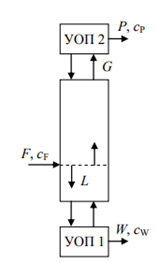
\includegraphics[scale=1]{latex/figures/figure1.png}
    \caption{Схема процесса разделения изотопов}
    Обозначения: $c_{P}$, $c_{F}$, $c_{W}$ – концентрации отбора, питания, отвала;
    
    $P$, $F$, $W$ – потоки отбора, питания, отвала
    \label{fig:cascade}
\end{figure}

Разделяемая бинарная смесь изотопов подаётся в среднюю часть колонны 
(рисунок ~\ref{fig:cascade}), в которой осуществляется противоточное движение фаз. 
Проходя последовательно ряд разделительных элементов, одна из фаз обогащается 
лёгким изотопом, а другая – тяжёлым. На концах колонны имеются специальные 
аппараты, которые предназначены для создания противоточного движения 
фаз путём перевода смеси изотопов из одной фазы в другую.

В стационарном режиме работы колонны справедливы следующие соотношения 
материального баланса:
\begin{equation}
    Fc_{F} = Pc_{P} + Wc_{W}
\end{equation}
\begin{equation}
    F = P + W
\end{equation}

В ряде случаев при большой высоте колонны и, исходя из различных практических 
особенностей организации разделительного процесса, колонну разбивают на 
несколько, образующие каскад колонн.
\newpage

\section{Методика проведения расчетов}
\newpage

\section{Практическая часть}
\subsection{Исходные данные для расчета}
Концентрация отбора $c_{P} =$ \var{concentraion_product};

Концентрация питания $c_{F} =$ \var{concentraion_feed};

Концентрация отвала $c_{W} =$ \var{concentraion_waste};

Температура $T =$ \var{temperature} $^{o}C$;

Поток отбора $P =$ \var{product_flow} $\dfrac{\text{кг}}{\text{год}}$;

Доля сокращения потока на одной ТТ $r =$ \var{flow_reduction_share} \%;

Количество ТТ в одной колонне $N =$ \var{number_theoretical_plates}.
\subsection{Расчет изменения изотопной концентрации по каскаду в 
стационарном режиме}
Поток отбора переведен из кг/год в моль/ч:

$P = \var{product_flow} \dfrac{\text{кг}}{\text{год}} = \dfrac{\var{product_flow} \dfrac{\text{кг}}{\text{год}}}{M} 
= \dfrac{\var{product_flow}\cdot\dfrac{1}{365\cdot 24} \dfrac{\text{кг}}{\text{ч}}}
{(7c_{P}+6(1-c_{P}))\cdot 10^{-3} \dfrac{\text{кг}}{\text{моль}}} \approx 
\var{product_flow_mol} \dfrac{\text{моль}}{\text{ч}}$

Рассчитано значение коэффициента разделения по формуле (\ref{koeff_separation}):
\begin{equation}\label{koeff_separation} 
    \alpha = 1 + \dfrac{4755}{T^{2}} - \dfrac{0,803}{T}
\end{equation}

$\alpha = 1 + \dfrac{4755}{(273+\var{temperature})^{2}} - \dfrac{0,803}{273+\var{temperature}} \approx \var{coefficient_separation}$

Рассчитано значение коэффициента обогащения по формуле (\ref{koeff_enrichment}):
\begin{equation}\label{koeff_enrichment}
    \varepsilon  = \alpha - 1
\end{equation}

$\varepsilon  = \var{coefficient_separation} - 1 = \var{coefficient_enrichment}$

По формуле (\ref{pr:number_theoretical_plates}) определено число 
теоретических тарелок:
\begin{equation}\label{pr:number_theoretical_plates}
n = 2\cdot (n_{\text{обог}} + n_{\text{рег}})
\end{equation}
\noindent где $n_{\text{обог}} = \dfrac{1}{\varepsilon}\ln\dfrac{c_{P}(1-c_{F})}{c_{F}(1-c_{P})}$, $n_{\text{рег}} = \dfrac{1}{\varepsilon}\ln\dfrac{c_{F}(1-c_{W})}{c_{W}(1-c_{F})}$

$n_{\text{обог}} = \dfrac{1}{\var{coefficient_enrichment}}\ln\dfrac{\var{concentraion_product}\cdot (1 - \var{concentraion_feed})}{\var{concentraion_feed}\cdot (1 - \var{concentraion_product})} \approx \var{number_theoretical_plates_enrichment}$

$n_{\text{рег}} = \dfrac{1}{\var{coefficient_enrichment}}\ln\dfrac{\var{concentraion_feed}\cdot (1 - \var{concentraion_waste})}{\var{concentraion_waste}\cdot (1 - \var{concentraion_feed})} \approx \var{number_theoretical_plates_depleted}$

$n = 2\cdot (\var{number_theoretical_plates_enrichment} + \var{number_theoretical_plates_depleted}) = \var{all_number_theoretical_plates}$

Количество колонн:

$n_{\text{кол}}^{all} = \dfrac{n}{N} = \dfrac{\var{all_number_theoretical_plates}}{\var{number_theoretical_plates}} \approx \var{number_column}$

Рассчитано изменение концентрации целевого изотопа в безотборном режиме по колоннам каскада с помощью формулы (\ref{eq:concentration1_change}):

\begin{equation}\label{eq:concentration1_change}
    c_{1}(n_{\text{кол}}) = \dfrac{\dfrac{c_{W}}{1-c_{W}}e^{\varepsilon Nn_{\text{кол}}}}{1 + \dfrac{c_{W}}{1-c_{W}}e^{\varepsilon Nn_{\text{кол}}}}
\end{equation}

\DTLforeach{concentration_c1}{\col=avar,\print=value}{
    $c_{1}(\col) = \dfrac{\dfrac{\var{concentraion_waste}}{1-\var{concentraion_waste}}e^{\var{coefficient_enrichment}\cdot \var{number_theoretical_plates}\cdot \col}}{1 + \dfrac{\var{concentraion_waste}}{1-\var{concentraion_waste}}e^{\var{coefficient_enrichment}\cdot \var{number_theoretical_plates}\cdot \col}} \approx \print$

}

Определена величина начального потока при работе каскада с заданным отбором по формуле (\ref{pr:initial_flow}):
\begin{equation}\label{pr:initial_flow}
    L_{\text{нач}} = kP\dfrac{c_{P} - c_{F}}{\varepsilon c_{F}(1 - c_{F})},
\end{equation}

\noindent где $k = \var{coefficient_cascade}$ - коэффициент для сшивки каскада по концентрации отвала.

$L_{\text{нач}} = \var{coefficient_cascade}\cdot \var{product_flow_mol}\cdot\dfrac{\var{concentraion_product} - \var{concentraion_feed}}{\var{coefficient_enrichment}\cdot\var{concentraion_feed}\cdot(1 - \var{concentraion_feed})} \approx \var{initial_flow} \text{ } \dfrac{\text{моль}}{\text{ч}}$

Сокращение потока $L$ по колоннам каскада:

\begin{equation}
    L_{\text{вых}}(n_{\text{кол}}) = L_{\text{нач}}(1 - r)^{Nn_{\text{кол}}}, n_{\text{кол}} = 1,2..n_{\text{кол}}^{all}
\end{equation}
\begin{equation*}
    L_{\text{вх}}(n_{\text{кол}}) = L_{\text{нач}}(1 - r)^{Nn_{\text{кол}}}, n_{\text{кол}} = 0,1,2..n_{\text{кол}}^{all}-1
\end{equation*}
\begin{equation}
    L_{\text{вх}}(n_{\text{кол}}) = L_{\text{нач}}(1 - r)^{N(n_{\text{кол}} - 1)}, n_{\text{кол}} = 1,2..n_{\text{кол}}^{all}
\end{equation}

Рассчитан средний поток для каждой колонны:
\begin{equation*}
L_{\text{ср}}(n_{\text{кол}}) = \dfrac{L_{\text{вых}}(n_{\text{кол}}) + L_{\text{вх}}(n_{\text{кол}})}{2}, n_{\text{кол}} = 1,2..n_{\text{кол}}^{all}
\end{equation*}
\begin{equation*}
    L_{\text{ср}}(n_{\text{кол}}) = \dfrac{L_{\text{нач}}(1 - r)^{Nn_{\text{кол}}} + L_{\text{нач}}(1 - r)^{N(n_{\text{кол}} - 1)}}{2}, n_{\text{кол}} = 1,2..n_{\text{кол}}^{all}
\end{equation*}
\begin{equation*}
    L_{\text{ср}}(n_{\text{кол}}) = \dfrac{L_{\text{нач}}(1 - r)^{Nn_{\text{кол}}} + L_{\text{нач}}(1 - r)^{Nn_{\text{кол}}}\cdot (1 - r)^{-N}}{2}, n_{\text{кол}} = 1,2..n_{\text{кол}}^{all}
\end{equation*}
\begin{equation*}
    L_{\text{ср}}(n_{\text{кол}}) = \dfrac{L_{\text{нач}}(1 - r)^{Nn_{\text{кол}}} \cdot (1 + (1 - r)^{-N})}{2}, n_{\text{кол}} = 1,2..n_{\text{кол}}^{all}
\end{equation*}
\begin{equation}
    L_{\text{ср}}(n_{\text{кол}}) = \dfrac{1}{2}L_{\text{нач}}(1 - r)^{Nn_{\text{кол}}} \cdot (1 + (1 - r)^{-N}), n_{\text{кол}} = 1,2..n_{\text{кол}}^{all}
\end{equation}

\DTLforeach{flow}{\col=avar,\print=value}{
    $L_{\text{ср}}(\col) = \dfrac{1}{2}\cdot \var{initial_flow}\cdot(1 - \var{flow_reduction_share}/100)^{\var{number_theoretical_plates}\cdot \col} \cdot (1 + (1 - \var{flow_reduction_share}/100)^{-\var{number_theoretical_plates}}) \approx$
    \begin{flushright}
    $\approx \print \text{ } \dfrac{\text{моль}}{\text{ч}}$
    \end{flushright}
    
}

Рассчитано изменение концентрации целевого изотопа по колоннам по уравнению (\ref{pr:concentration_c2}):
\begin{equation}\label{pr:concentration_c2}
    c_{2}(n_{\text{кол}}) = \dfrac{x_{1} + \dfrac{x_{1} - c_{P}}{c_{P} - x_{2}} e^{Nn_{\text{кол}}\varepsilon (x_{1} - x_{2})}x_{2}}{1 + \dfrac{x_{1} - c_{P}}{c_{P} - x_{2}} e^{Nn_{\text{кол}}\varepsilon (x_{1} - x_{2})}}
\end{equation}

\noindent где $x_{1,2} = \dfrac{1}{2}(1 + \dfrac{P}{L\varepsilon})\pm \sqrt{\dfrac{1}{4}(1 + \dfrac{P}{L\varepsilon})^{2} - \dfrac{P}{L\varepsilon}c_{P}}.$

\DTLforeach{concentration_c2}{\col=avar,\xin=x1,\xinn=x2,\print=value}{
    $x_{1,2}(\col) = \dfrac{1}{2}(1 + \dfrac{\var{product_flow_mol}}{\varflow{\col}\cdot\var{coefficient_enrichment}})\pm$
    \begin{flushright}
    $\pm \sqrt{\dfrac{1}{4}(1 + \dfrac{\var{product_flow_mol}}{\varflow{\col}\cdot\var{coefficient_enrichment}})^{2} - \dfrac{\var{product_flow_mol}}{\varflow{\col}\cdot\var{coefficient_enrichment}}\cdot\var{concentraion_product}}\approx \left [ \begin{gathered} 
        \xin\\ 
        \xinn\\ 
      \end{gathered}\right. $
    \end{flushright}

    $c_{2}(\col) = \dfrac{\xin + \dfrac{\xin - \var{concentraion_product}}{\var{concentraion_product} - \xinn} e^{\var{number_theoretical_plates}\cdot\col\cdot\var{coefficient_enrichment}\cdot(\xin - \xinn)}\cdot\xinn}{1 + \dfrac{\xin - \var{concentraion_product}}{\var{concentraion_product} - \xinn} e^{\var{number_theoretical_plates}\cdot\col\cdot\var{coefficient_enrichment} (\xin - \xinn)}}\approx $
    \begin{flushright}
    $\approx\print$
    \end{flushright}

}
В таблицах \ref{tab:concP0} и \ref{tab:concP} приведены результаты расчета изменения концентрации по колоннам каскада в режимах без отбора и с отбором.
\begin{table}[hbtp]
    \caption{Изменение концентрации $^{7}$Li по колоннам каскада для безотборного режима}
    \vspace{-0.2cm}
    \label{tab:concP0}
    \begin{tabularx}{\textwidth}{|C{0.5}|C{0.5}|}
        \hline
        $n_{\text{кол}}$&$c_{1}$\\
        \hline
        \DTLforeach{concentration_c1}{\col=avar,\print=value}{
            \col&\print\\
            \hline
        }
    \end{tabularx}
\end{table}

\begin{table}[hbtp]
    \caption{Изменение концентрации $^{7}$Li по колоннам каскада для режима с отбором}
    \vspace{-0.2cm}
    \label{tab:concP}
    \begin{tabularx}{\textwidth}{|C{0.5}|C{0.5}|}
        \hline
        $n_{\text{кол}}$&$c_{1}$\\
        \hline
        \DTLforeach{concentration_c2}{\col=avar,\print=value}{
            \col&\print\\
            \hline
        }
    \end{tabularx}
\end{table}

График изменения концентрации в режимах с отбором и без представлен на рисунке \ref{fig:concentraion_change}.
\begin{figure}[hbtp]
    \centering
    \captionsetup{justification=centering}
    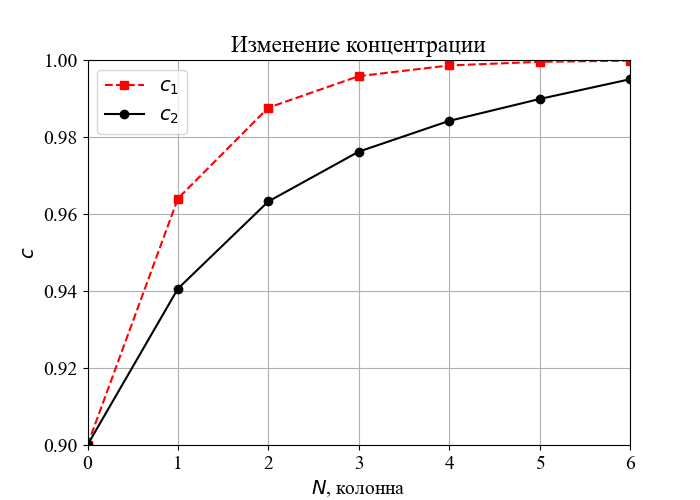
\includegraphics[scale=1]{latex/figures/concentration_change.png}
    \caption{Изменение концентрации по колоннам каскада}
    $c_{1}$ -- без отбора, $c_{2}$ -- с отбором
    \label{fig:concentraion_change}
\end{figure}

Определены величины потоков отвала и питания из уравнения материального баланса (\ref{pr:system_material}):
\begin{equation}\label{pr:system_material}
    \begin{cases}
    Fc_{F} = Pc_{P} + Wc_{W}\\
    F = P + W
    \end{cases}
\end{equation}

В данной системе уравнений неизвестными являются потоки питания ($F$) и отвала ($W$).
\begin{equation*}
    \begin{cases}
    Pc_{F} + Wc_{F} = Pc_{P} + Wc_{W}\\
    F = P + W
    \end{cases}
\end{equation*}
\begin{equation*}
    \begin{cases}
    W(c_{F} - c_{W}) = P(c_{P} - c_{F})\\
    F = P + W
    \end{cases}
\end{equation*}
\begin{equation*}
    \begin{cases}
    W = P\dfrac{c_{P} - c_{F}}{c_{F} - c_{W}}\\
    F = P + W
    \end{cases}
\end{equation*}
\begin{equation}
    W = P\dfrac{c_{P} - c_{F}}{c_{F} - c_{W}}
\end{equation}
\begin{equation}
    F = P + W
\end{equation}

$W = \var{product_flow_mol}\cdot\dfrac{\var{result_concentartion_product} - \var{concentraion_feed}}{\var{concentraion_feed} - \var{result_concentartion_waste}} \approx \var{result_waste}\text{ }\dfrac{\text{моль}}{\text{ч}}$

$F = \var{product_flow_mol} + \var{result_waste} = \var{result_feed}\text{ }\dfrac{\text{моль}}{\text{ч}}$

Принципиальная схема получившегося каскада приведена на рисунке \ref{fig:cascade_all}. Сплошными стрелками показано движение гидроксида лития, пунктиром – амальгамы.
\begin{figure}[hbtp]
    \centering
    \captionsetup{justification=centering}
    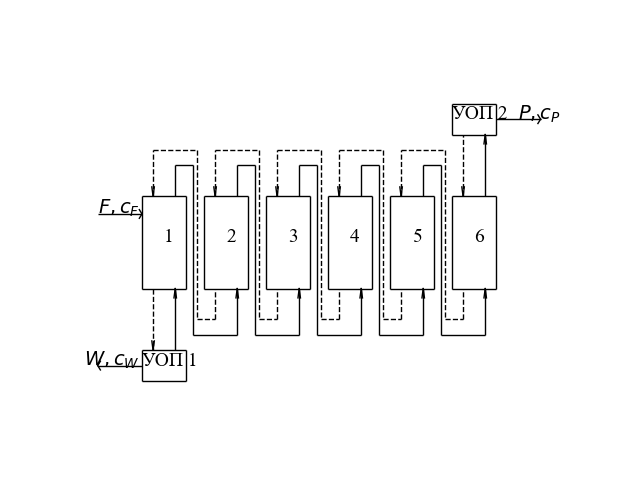
\includegraphics[scale=1]{latex/figures/cascade.png}
    \caption{Принципиальная схема каскада}
    \label{fig:cascade_all}
\end{figure}

Каскад состоит из шести колонн изотопного обмена с питанием на первой и двух узлов обращения потоков.

В узле обращения потоков 1 происходит реакция разложения амальгамы:
\begin{equation}
    Li_{n}Hg + H_{2}O \rightarrow LiOH + Hg + \dfrac{1}{2}H_{2}
\end{equation}

Образовавшийся гидроксид лития поступает в колонну изотопного обмена 1, где движется противотоком амальгаме.

В узле обращения потоков 2 протекает реакция:

\begin{equation}
    LiOH + Hg \rightarrow Li_{n}Hg + H_{2}O + \dfrac{1}{2}O_{2}
\end{equation}

Обращение проводят в электролизере с ртутным катодом \cite{mushkin}. Образовавшаяся в электролизере амальгама поступает в колонну изотопного обмена 6, где она движется противотоком к раствору.

Амальгама обогащается по легкому изотопу $^{6}$Li, раствор лития – по тяжелому $^{7}$Li.
\newpage

\section*{Выводы}
\begin{enumerate}
\item Проведен расчет изменения концентрации $^{7}$Li по колоннам каскада 
в режимах без отбора и с отбором при заданных параметрах его работы для 
амальгамно-обменного способа. Построены график изменения концентрации 
$^{7}$Li в обоих режимах работы каскада и принципиальная схема полученного 
каскада.

\item Рассчитано, что для обеспечения целевой концентрации на выходе из 
каскада колонн в безотборном режиме необходимо минимально три колонны.

\item Показано, что в режиме без отбора концентрация по $^{7}$Li на выходе 
из каскада колонн, состоящей из 6 обменных колонн, 0,99984. 

\item Определено, что необходимо увеличить минимальный начальный поток 
в 1,576 раз для сшивки каскада по концентрации отвала. 

\item Установлено, что скорость изменения концентрации по колоннам каскада 
для режима без отбора больше, чем для режима с отбором.

\item Определены потоки питания F = 9,30749 моль/ч и 
отвала W = 6,85956 моль/ч.
\end{enumerate}


\newpage
\addcontentsline{toc}{section}{Список использованных источников}
\begin{thebibliography}{2}
\bibitem{mukhin}
Мухин К.Н. Экспериментальная ядерная физика. В двух томах. Т. 1. Физика атомного ядра. Учебник для вузов. Изд. 3-е М., Атомиздат, 1974 г., 584 с.
\bibitem{rocus}
РД-07-15-2002. Федеральный надзор России по ядерной и радиационной безопасности [Текст]. -- Введ. 2003-05-10. -- М.:Гостатомнадзор России.
\bibitem{kondratiy}
Кондратьев В.Н. Кинетика химических газовых реакций, М.: АН СССР, 1958. — 693 с.
\bibitem{gik}
Источники Гамма - излучения: [Электронный ресурс] // Изотоп Ростатом. URL:  \url{http://www.isotop.ru/files/treecontent/nodes/attaches/0/95/noname..pdf}. (Дата обращения 15.04.2022).
\bibitem{steel12}
Сталь марки 12Х18Н10Т: [Электронный ресурс] // Центральный металлический портал. URL: \url{https://metallicheckiy-portal.ru/marki_metallov/stk/12X18H10T} (Дата обращения 15.04.2022).
\bibitem{steel02}
Сталь марки AISI316: [Электронный ресурс] // Центральный металлический портал. URL: \url{https://metallicheckiy-portal.ru/marki_metallov/stn/AISI316} (Дата обращения 15.04.2022).
\bibitem{geant4}
Geant4 A simulation toolkit: [Электронный ресурс]. URL:  \url{https://geant4.web.cern.ch/}. (Дата обращения 15.02.2022).
\bibitem{PrataC++}
Стивен Прата. Язык программирования C++ (C++11). Лекции и упражнения, 6-е издание — М.: Вильямс, 2012. — 1248 с.
\end{thebibliography}


\end{document}